\documentclass[conf]{new-aiaa}
%\documentclass[journal]{new-aiaa} for journal papers
\usepackage[utf8]{inputenc}

\usepackage{graphicx}
\usepackage{amsmath}
\usepackage[version=4]{mhchem}
\usepackage{siunitx}
\usepackage{longtable,tabularx}
\usepackage{footnote}
\usepackage{mhchem}
\usepackage{physics}
\usepackage{array,makecell,booktabs}
\newcolumntype{M}[1]{>{\centering\arraybackslash}m{#1}}
\usepackage[super]{nth}
\makesavenoteenv{tabular}
\setlength\LTleft{0pt}

\graphicspath{{figures/}}

\begin{document}

\section{Cost Model}

The TRANSCOST 8.2 model was implemented to evaluate the costs of different first stage reuse strategies \cite{transcost}. TRANSCOST is a top-down cost estimating model that utilizes historical data for similar projects to estimate the cost of launch vehicle elements. A series of cost estimation relationships (CERs) of the form $C = a M^x$ relate the mass $M$ of launch vehicle elements to their production costs using the empirically fitted parameters $a$ and $x$. Costs of all launch vehicle elements are then summed to determine the total launch vehicle production cost. 

The cost and performance models are linked through the launch vehicle element masses. For a given payload mass, the performance model can estimate the mass of launch vehicle elements for various first stage reuse strategies. These masses are then used with the cost model to estimate the production cost and cost per flight of those strategies. 

\subsection{Cost Model Description}

The TRANSCOST model considers three separate cost areas for launch vehicles: development, production, and operations costs \cite{transcost}. The cost per flight of a launch vehicle is the cost paid by the launch service provider for each flight, which includes production and operations costs only. The price per flight is the price paid by a customer to the launch service provider. This includes production and operations costs, as well as profit for the launch service provider and a potential development amortization charge. It should be noted, however, that typically development costs are funded by government contracts or third party investors, such as for the TODO launch vehicles [TODO citation]. In these cases, a development amortization charge is not included as part of the price per flight.

It is interesting to look at the breakdown of costs in the cost per flight of a launch vehicle. Consider a two stage fully expendable launch vehicle utilizing kerosene and liquid oxygen propellants to carry a 10,000 kg payload to LEO. The cost per flight breakdown for such a launch vehicle can be seen in Fig. \ref{fig:expendable_cost_breakdown}. 

\begin{figure}[hbt!]
    \centering
    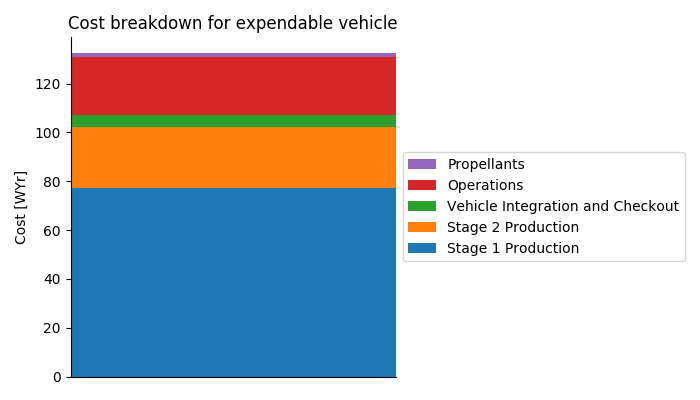
\includegraphics[width=0.7\textwidth]{../../lvreuse/analysis/combined/plots/expendable_cost_breakdown}
    \caption{\label{fig:expendable_cost_breakdown} Cost per flight breakdown for two stage fully expendable vehicle.}
\end{figure}

For this launch strategy -- and similarly for most fully expendable launch vehicle strategies -- the cost per flight is dominated by the first stage production costs. These large first stage production costs motivate strategies for first stage reusability, which would allow the first stage production cost to be amortized over a number of flights, therefore potentially reducing the total cost per flight. 

quantification of uncertainty - CER data extraction/confidence bounds

\subsection{Validation of Cost Model}

In order to validate the TRANSCOST model, the prices per flight for several current launch vehicles were evaluated with the model and compared to their actual advertised launch prices. As with the performance model, uncertainty in the cost model is accounted for using Monte Carlo methods. Credible range estimates for various cost parameters are used to establish parameter distributions. These distributions are then sampled to evaluate the cost model, generating a collection of cost model outputs that represent a range of credible cost estimates.

\begin{figure}[hbt!]
    \centering
    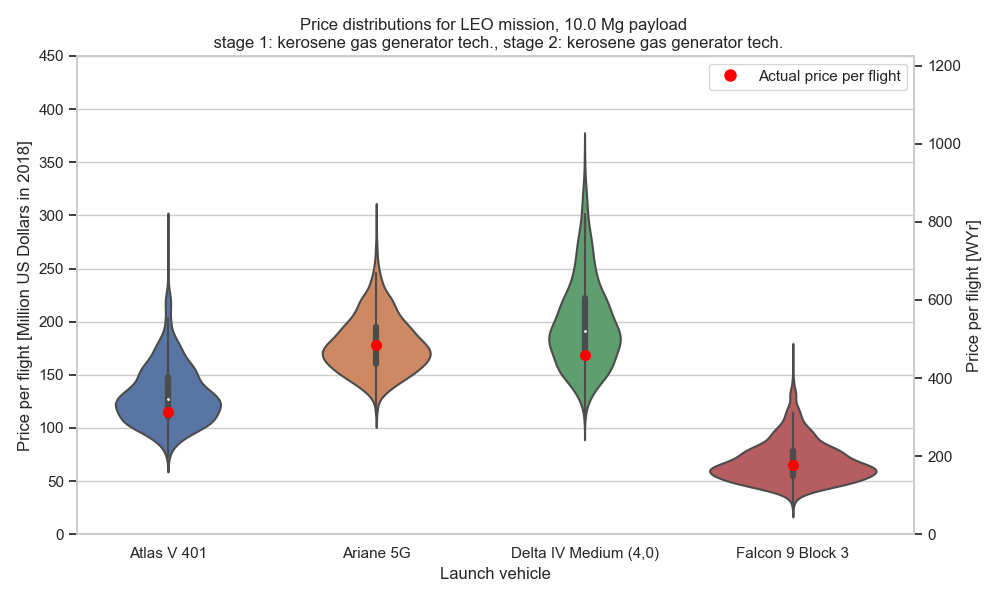
\includegraphics[width=\textwidth]{../../lvreuse/analysis/cost/plots/vehicle_ppf_validation}
    \caption{\label{fig:vehicle_ppf_validation} TODO caption.}
\end{figure}

\bibliography{first_stage_recovery}

\end{document}